
\medskip

Pour le mariage de Dominique et Camille, le pâtissier propose deux pièces montées constituées de
gâteaux de tailles et de formes différentes.
\begin{center}
\begin{tabularx}{\linewidth}{|X|m{4cm}|}\hline
\textbf{La tour de Pise :}

La première pièce montée est constituée d'un empilement de
4~gâteaux de forme cylindrique, de même hauteur et dont le
diamètre diminue de $8$~cm à chaque étage.

Le gâteau du bas a pour diamètre $30$~cm et pour hauteur $6$~cm.&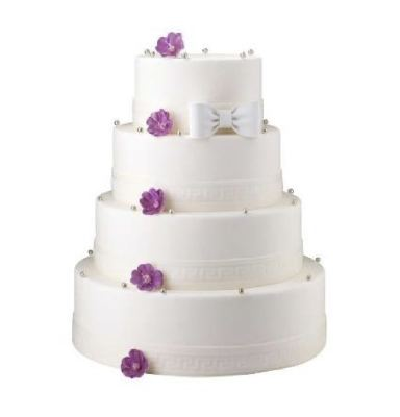
\includegraphics[width=3.9cm]{gateau_1}\\ \hline
\textbf{La tour Carrée :}

La deuxième pièce montée est constituée d'un empilement de
$3$ pavés droits à base carrée de même hauteur. La longueur du
côté de la base diminue de $8$~cm à chaque étage.

La hauteur des gâteaux est $8$~cm ; le côté de la base du gâteau
du bas mesure $24$~cm.&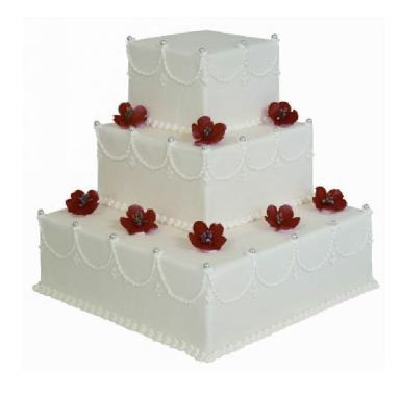
\includegraphics[width=3.9cm]{gateau_2}\\ \hline
\end{tabularx}
\end{center}
\medskip

Tous les gâteaux ont été confectionnés à partir de la recette ci-dessous qui donne la quantité des
ingrédients correspondant à $100$~g de chocolat.

\begin{center}
\begin{tabularx}{\linewidth}{|X|X|}\hline
\textbf{Recette du gâteau pour 100 g de chocolat :}& \begin{itemize}
\item 65 g de sucre
\item 2 oeufs
\item 75 g de beurre
\item 30 g de farine
\end{itemize}\\ \hline
\end{tabularx}
\end{center}

\begin{enumerate}
\item Quel est le ratio (masse de beurre : masse de chocolat) ? Donner le résultat sous forme de fraction irréductible.

\item  Calculer la quantité de farine nécessaire pour $250$~g de chocolat noir suivant la recette ci-dessus.

\item Calculer la longueur du côté de la base du plus petit gâteau de la tour Carrée.

\item  Quelle est la tour qui a le plus grand volume ? Justifier votre réponse en détaillant les calculs.

\end{enumerate}

On rappelle que le volume $V$ d'un cylindre de rayon $r$ et de hauteur $h$ est donné par la formule:

\[V = \pi \times  r^2 \times h.\]

\bigskip

